\documentclass[11pt,a4paper]{article}
\usepackage[a4paper, margin=1.3in]{geometry}
\usepackage{mathtools}
\usepackage{graphicx}
\usepackage{fancyhdr}
\pagestyle{fancy}
\fancyhf{}
\lhead{AI Planning}
\rhead{Exercise Sheet 6}
\lfoot{Axel Perschmann, Tarek Saier, dd.12.2014}
\rfoot{Page \thepage\ of n}
\renewcommand{\headrulewidth}{0.3pt}
\renewcommand{\footrulewidth}{0.3pt}
\setlength\parindent{0pt}

\newcommand{\h}[0]{\text{--}}

\begin{document}
\begin{center}
\Huge{\textbf{AI Planning}}\\
\LARGE{\textbf{Exercise Sheet 6}}
\end{center}
\vspace{2cm}
\begin{tabular}{ll}
Date: & dd.11.2014\\
Students: & Axel Perschmann, Tarek Saier
\end{tabular}

\section*{Exercise 6.1}
foo

\section*{Exercise 6.2}
<<<<<<< HEAD
Example for an overestimation:
\begin{figure}[h!]
\centering
\caption{Over Estimation of $h_{add}$}
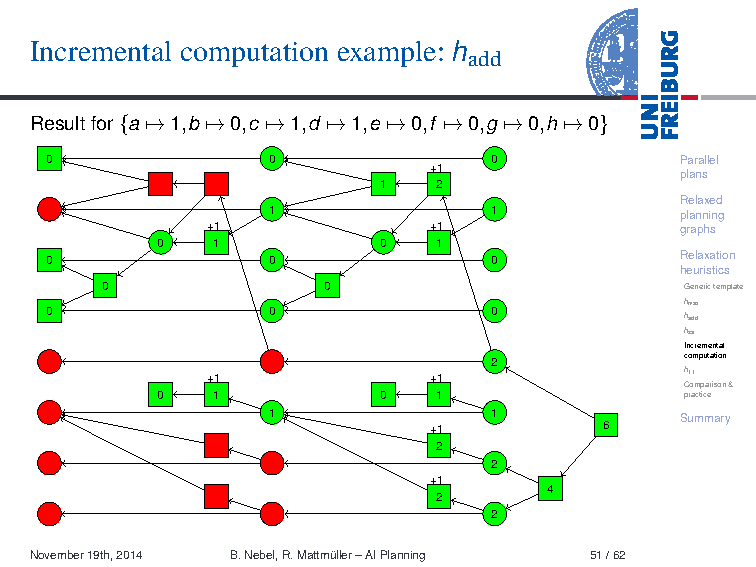
\includegraphics[scale=1]{aip08-handout51}
\end{figure}
=======
\begin{tabular}{l} % to force the text part and the graph to appear on the same page
Relaxed planning graph with depth 3. (Sparse labeling due to technical restrictions.)\\
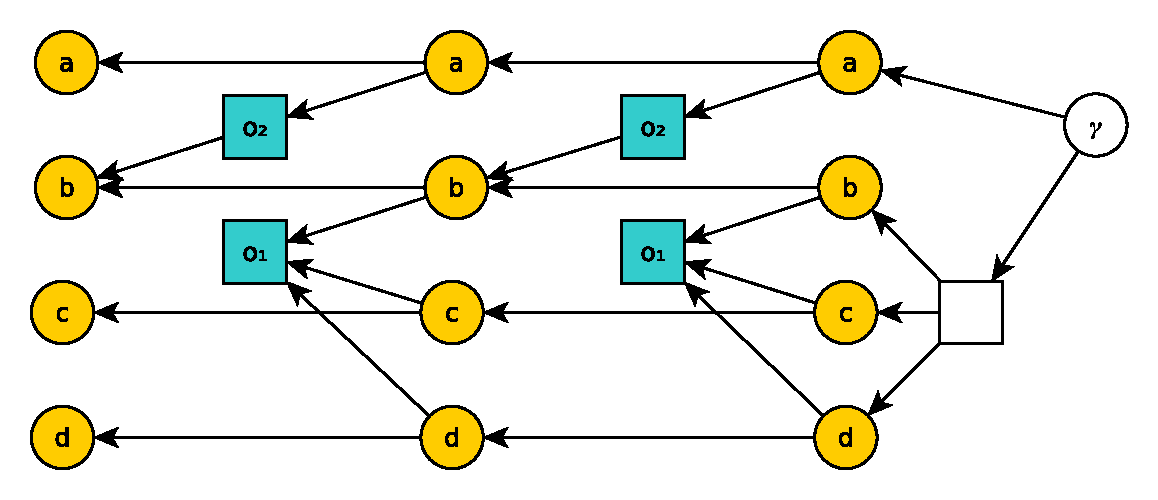
\includegraphics[scale=0.5]{g62}\\
\end{tabular}

\begin{tabular}{l} % to force the text part and the graph to appear on the same page
Depth 2, $h_{add}(s)=3$\\
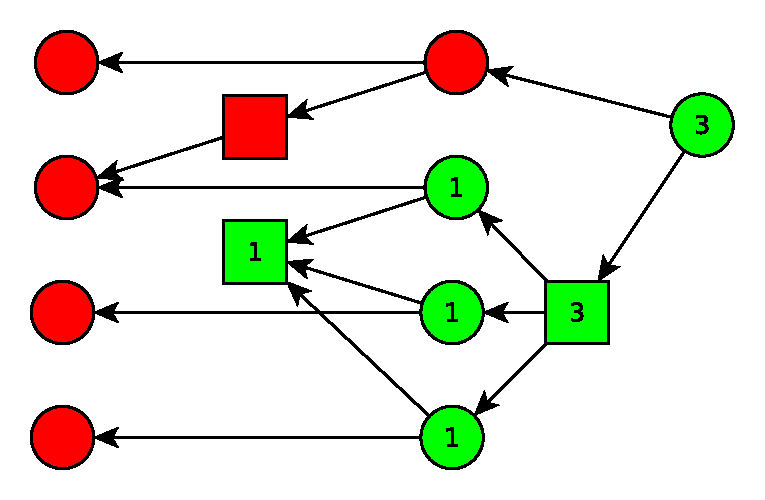
\includegraphics[scale=0.5]{g622}\\
\end{tabular}

\begin{tabular}{l} % to force the text part and the graph to appear on the same page
Depth 3, $h_{add}(s)=2$\\
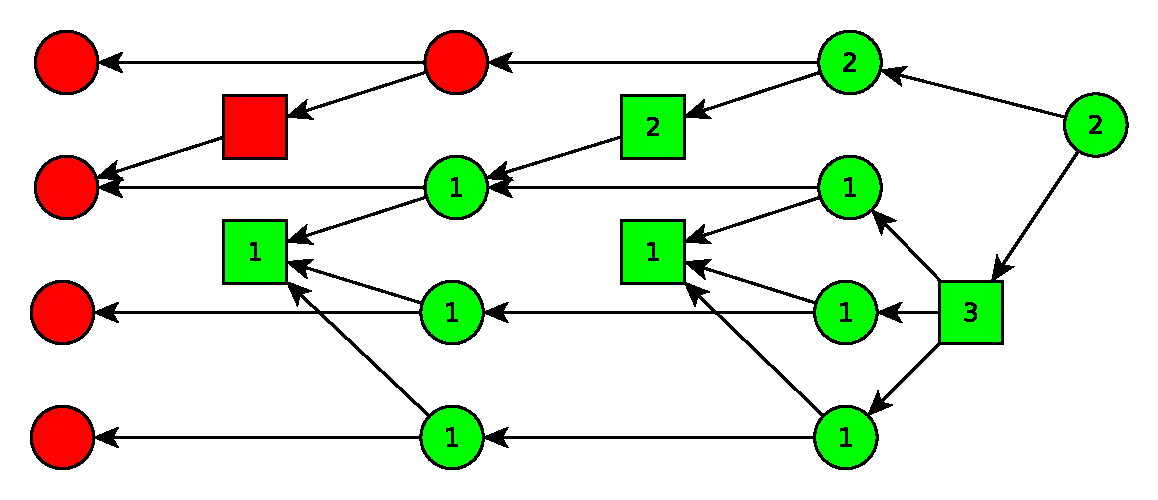
\includegraphics[scale=0.5]{g621}\\
\end{tabular}
>>>>>>> 693ecaec3aa6213dc410849f6c6b980bb9c753bd

\section*{Exercise 6.3}
\begin{tabular}{l} % to force the text part and the graph to appear on the same page
Relaxed planning graph with depth 3. (Sparse labeling due to technical restrictions.)\\
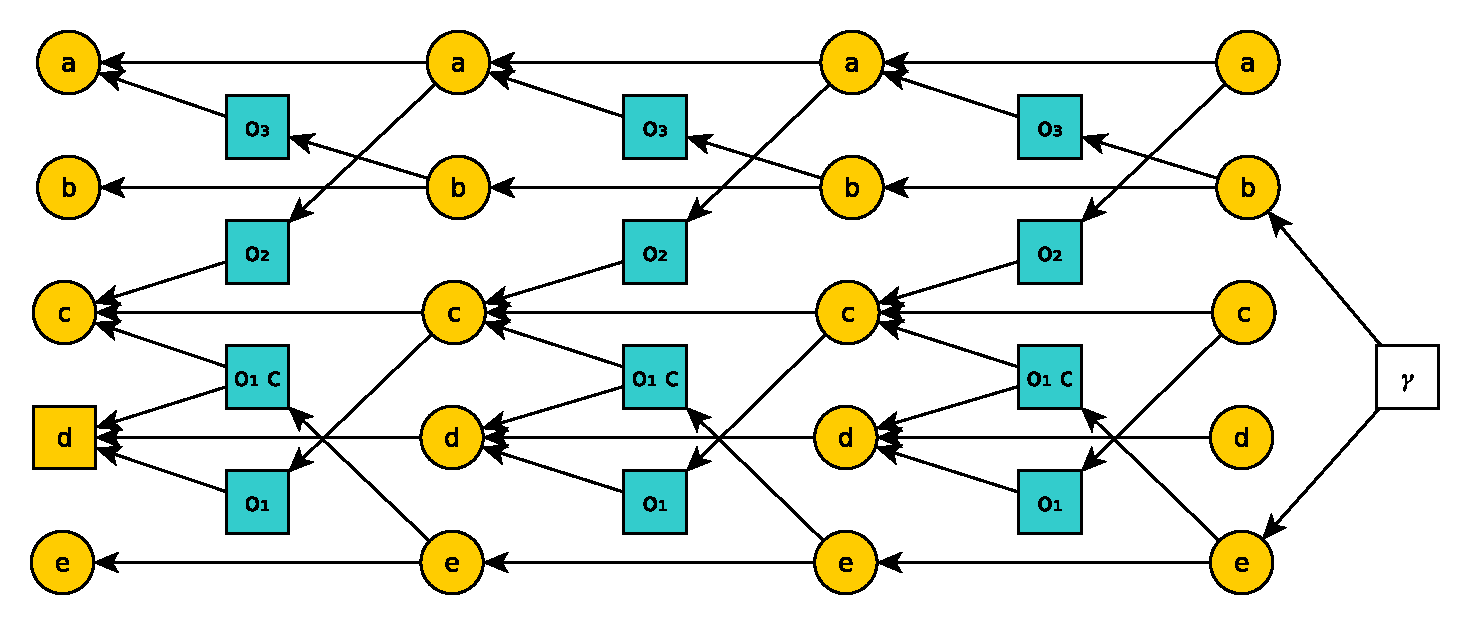
\includegraphics[scale=0.5]{g63}\\
\end{tabular}

\begin{tabular}{l} % to force the text part and the graph to appear on the same page
\textbf{(a)} $h_{max}(s)=3$\\
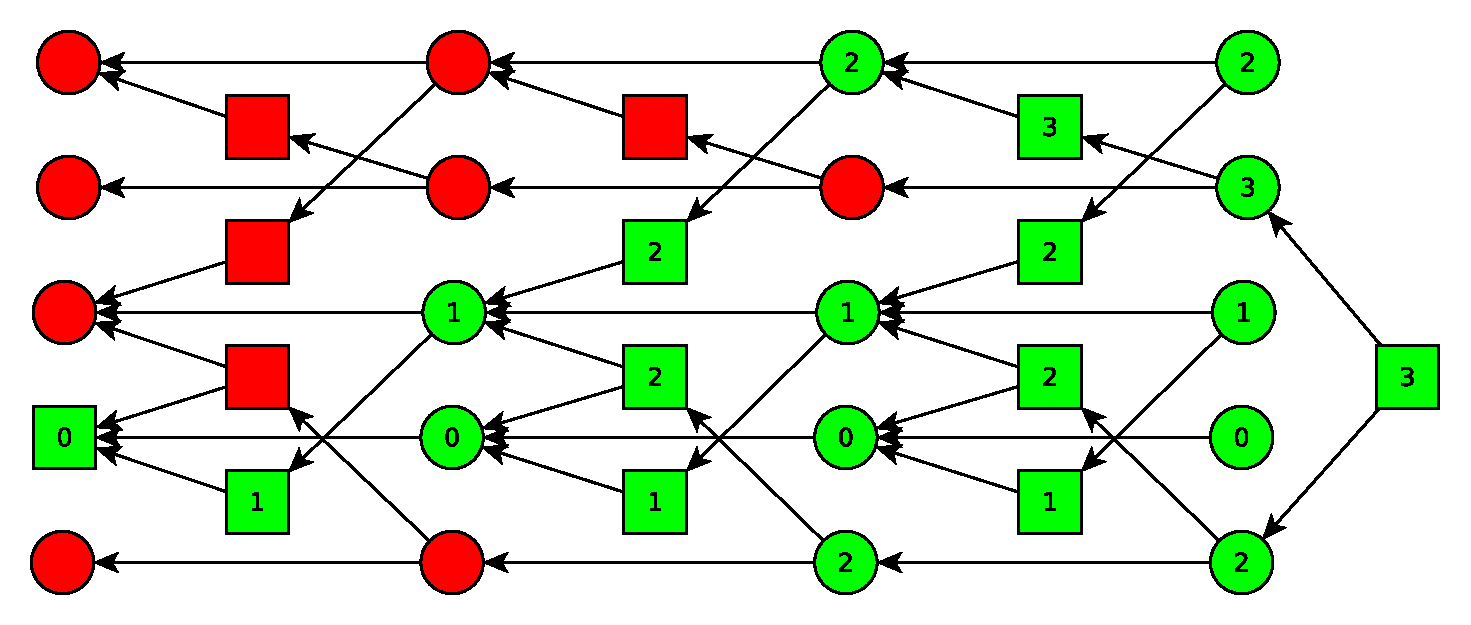
\includegraphics[scale=0.5]{g63a}\\
\end{tabular}

\begin{tabular}{l} % to force the text part and the graph to appear on the same page
\textbf{(b)} $h_{add}(s)=5$\\
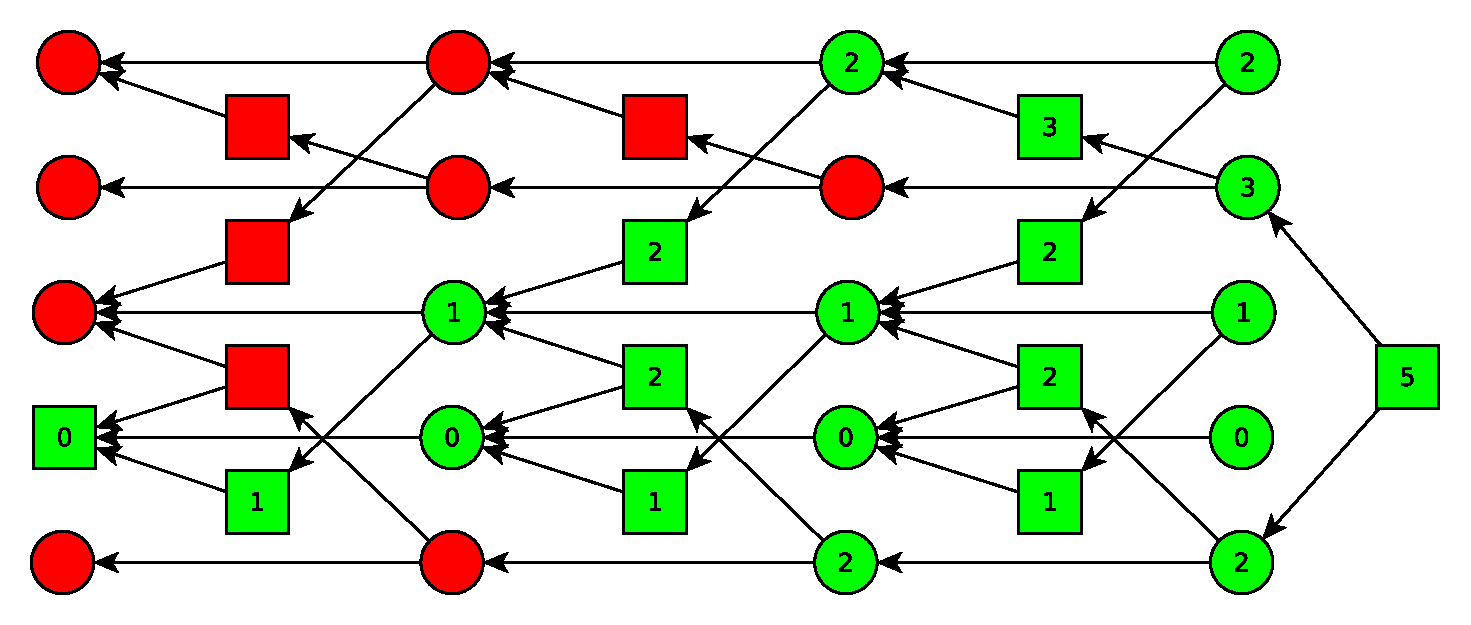
\includegraphics[scale=0.5]{g63b}\\
\end{tabular}

\begin{tabular}{l} % to force the text part and the graph to appear on the same page
\textbf{(c)} $h_{sa}(s)=4$\\
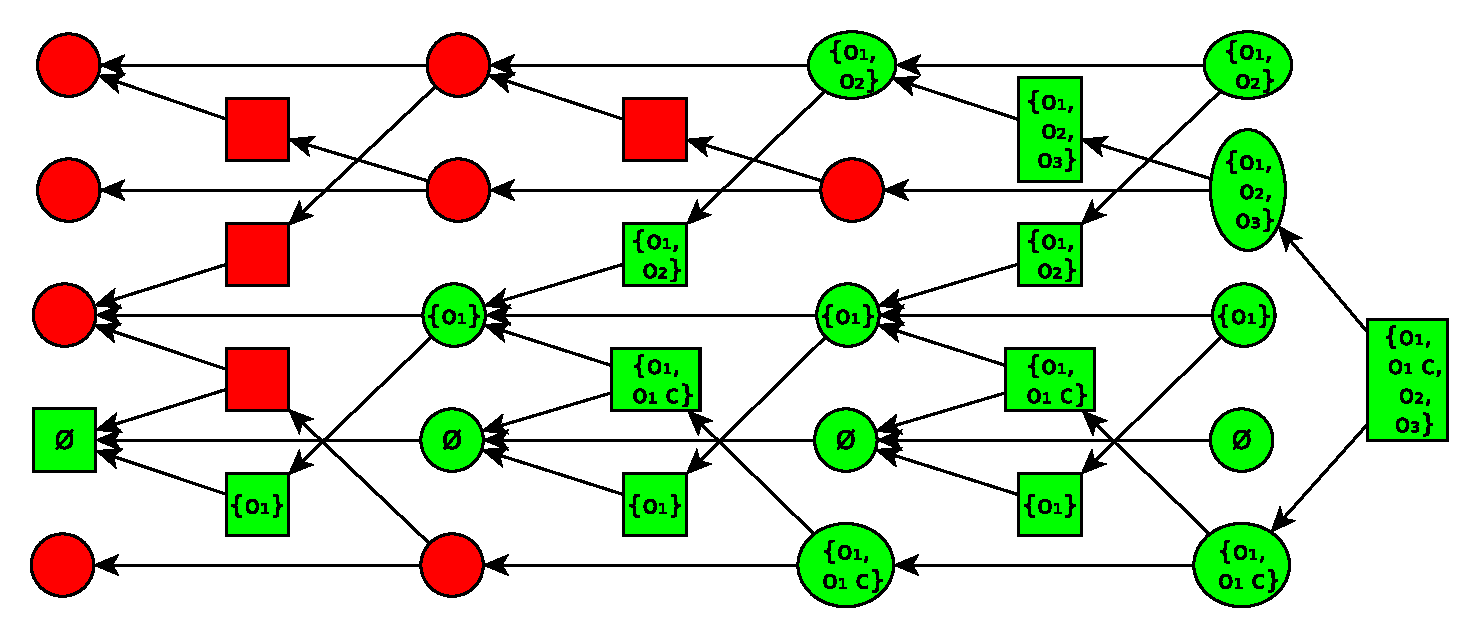
\includegraphics[scale=0.5]{g63c}\\
\end{tabular}

\begin{tabular}{l} % to force the text part and the graph to appear on the same page
\textbf{(d)} $h_{FF}(s)=4$\\
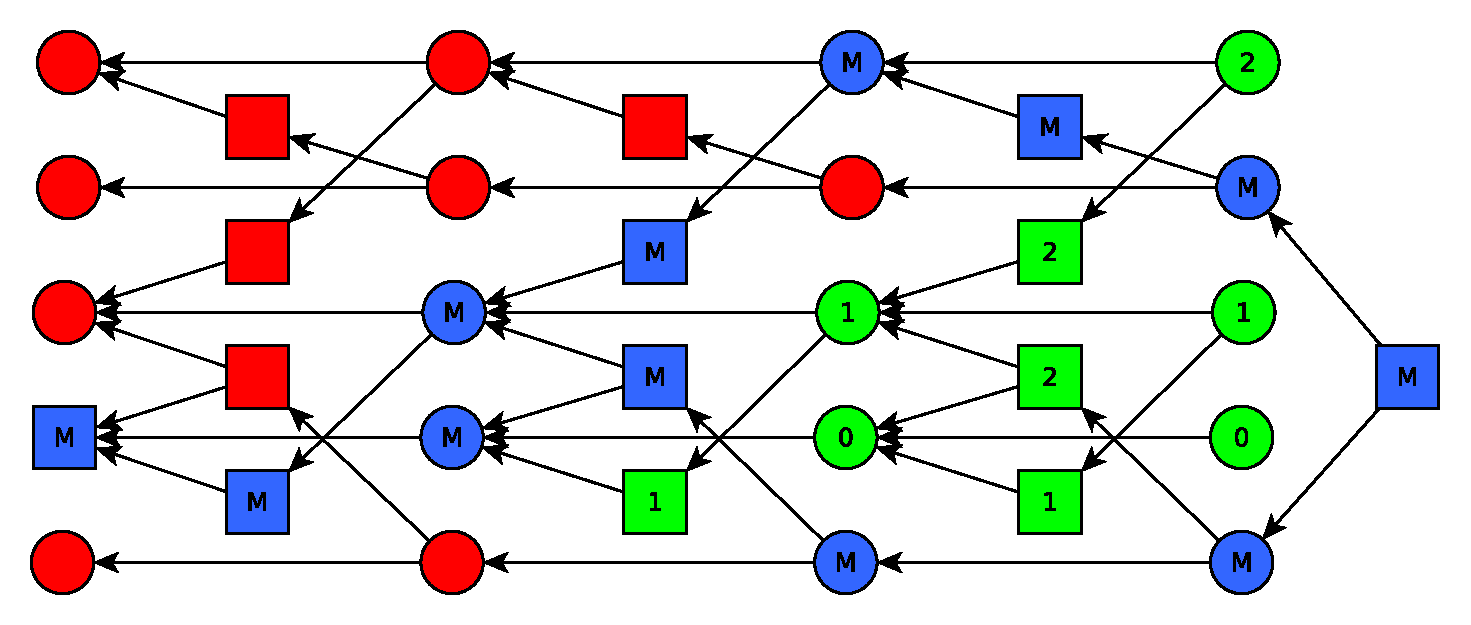
\includegraphics[scale=0.5]{g63d}\\
\end{tabular}

\end{document}
